
%%%%%% pre start>
% variables declarations
\def\docTitle{SuPong}
\def\docSubtitle{Project documentation}
\def\docAuthors{\textit{The F-Team}\\ Fabian Page \\Fabio Bernasconi}

\def\imgPrefix{images}

\documentclass[12pt,a4paper,oneside]{scrartcl}

\usepackage{ae}
\usepackage{geometry}
\usepackage{color, colortbl}


%% language specific and text handling stuff
%\usepackage{ngerman}  % use german labels for content, references etc.
\usepackage[ansinew]{inputenc} % let us write german/french special chars
\usepackage{textcomp} % for symbols like celsius etc.
%\usepackage{soul} % highlighting with \hl{}


%% listings
\usepackage{listings}

%% table packages
\usepackage{longtable}
\usepackage{multirow}


%% use the makeindex package
\usepackage{makeidx}
\makeindex


%% header packages
\usepackage{fancyhdr}


%% pdf processing
\usepackage{ifpdf}


%% graphics stuff
\usepackage{wrapfig} % wrapping text around images

% This makes images possible both in latex and pdftex 
\newif\ifpdf
\ifx\pdfoutput\undefined
   \pdffalse 
\else
   \pdfoutput=1
   \pdftrue
\fi

\ifpdf
   \usepackage[pdftex]{graphicx}
\else
   \usepackage{graphicx}
\fi

\usepackage{rotating}

%% some color definitions for pdflatex
% this is where the magic happens (propper pdf referencing)
\definecolor{LinkColor}{rgb}{0.8,0.1,0.1} % nice links in pdfs
\usepackage[%
        pdftex,%
        backref,%
        pagebackref]%
				{hyperref}
\hypersetup{colorlinks=true,%
        linkcolor=LinkColor,%
        citecolor=LinkColor,%
        filecolor=LinkColor,%
        menucolor=LinkColor,%
        pagecolor=LinkColor,%
        urlcolor=LinkColor}


%% format definitions
\setlength{\unitlength}{1mm}
\setlength{\parindent}{0mm} % no indentation for \par
\setlength{\parskip}{1ex plus 0.5ex minus 0.2ex}


%% paper border definitions
\geometry{inner=2.2cm,top=2.5cm}


% \usepackage{datetime}
% \ddmmyyyydate
% \renewcommand{\dateseparator}{.}


%% versioning
%\usepackage{svninfo}

% header stuff
\pagestyle{fancyplain}
\lhead[Fabian Page, Fabio Bernasconi\\]{Fabian Page, Fabio Bernasconi\\}
\chead[]{}
\rhead[Microcontroller Programming\\Project
documentation]{Microcontroller Programming\\Project documentation}
\cfoot[\thepage]{\thepage}  

%%%%%% <pre end


\begin{document}


% --- config - start --- 
\def\versioningFileName{versioning.tex}
\def\mySpace{ }

\newcommand{\Hrule}{\rule{\linewidth}{1mm}}
% --- config - end --- 

\thispagestyle{empty} % no headings, no footer 

\date{\today}
\enlargethispage{2cm}

\small\textsf{
    \begin{picture}(0,0)(0,0)
        \put(0,-5){
\includegraphics[height=2cm]{images/unibern_logo.png}} 
        \put(65,0){
\includegraphics[height=1cm]{images/ti-e.jpg}} 
        \put(30,0){
\includegraphics[height=1cm]{images/logo_bfh_new.png}}
    \end{picture}
}

\vspace*{6cm}

\Hrule

\begin{flushright}
    {
     \bfseries{\huge \docTitle}\\[8mm] 
     {\large \docSubtitle}\\
    }
\end{flushright}

\Hrule

\vspace*{1.5cm}
\begin{flushright}
	{
		by \docAuthors
	}
\end{flushright}

\vspace{\stretch{2}}
\begin{flushright}
%\rule{\linewidth}{0.1mm}
\tiny\textit{last Update \today} \hfill \\
\end{flushright}

%\begin{picture}(0,0)(0,0)
%	\put(35,100){\input{\includeDir/info-table.tex}}
%\end{picture}


\newpage
\thispagestyle{empty} % no headings, no footer
\tableofcontents

\newpage
\section{Introduction}
This document describes the implementation of the SuPong game for the Keil ARM
STR9x board. SuPong is a project written for the Microcontroller
Programming course that is part of the Biomedical Engineering Master at the
University of Bern.

\section{SuPong - the game}
SuPong is an implementation of the well known video game pong
\footnote{see for a description of the game
\url{http://en.wikipedia.org/wiki/Pong}}. The implementation of the game itself
was straight forward and thus will not be considered any further in this
document although some parts of the logic are incomplete.

\section{STR9x Implementation}
Prior to implement the game for the STR9x, the project team decided to write an
x86 version of it (without input handling though). This decision was taken
because testing of the game implementation itself was a lot easier on a x86
platform than it is on the the Keil STR9x kit. 

The display of the Keil STR9x board is only 2x16 characters large (small). To
make the game more fun to play the project team decided to use a second board.
Using two boards the screen dimensions doubles, that is it grows to 4x16
characters.

The boards communicate over a network. The project team used the TCP/IP
stack implementation of the easyweb demo pack. Using the Keil RTX would have
been easier since the easyweb TCP/IP implementation is kind of a hack.
This resulted in a long and painful development time for the network realted
stuff. Once the boards are running the slave tries to connect to the server. 
Thus it is important that the master is running before the slave does. After the
initialization phase the master and slave alternatively send and receive a
``state token''. The state token contains the complete game state.

\newpage
\section{Developer Documentation}
\label{sec_devdoc}
This section gives a short introduction on how to setup the development
environment that was used to develop the SuPong, how to flash the board or how
to compile a x86 version of the game.

\subsection{Development Environment}
Eclipse CDT\footnote{\url{http://www.eclipse.org/cdt/}} and $\mu$Vision
IDE\footnote{\url{http://www.keil.com}}. See \ref{sec_compx86} and
\ref{sec_str9ver} for platform setup.

\subsubsection{Directory structure}
\begin{itemize}
  \item SuPong
  \begin{itemize}
	  
	  \item src  ; all the source files except the keil libs
	  \begin{itemize}
	  	\item core
		  \begin{itemize}
		  	\item engine.h   ; main include file, game logic
		  	\item engine.c	 
		  	\item supong.h   ; game structs and the like
		  	\item supong.c
		  	\item types.h    ; some type definitions
		  \end{itemize}
      
      \item x86
	      \begin{itemize}
	        \item renderer/consoleRenderer.h  ; provides functions for game
	        rendering
	        \item renderer/consoleRenderer.c
            \item main.c  ; main entry point
            \item README  ; some notes for the x86 development platform
          \end{itemize}
      
      \item str9
	      \begin{itemize}
	        \item str9Renderer.h
	        \item str9Renderer.c
            \item main.c  ; main entry point
	        \item \ldots
          \end{itemize}
      \end{itemize}
	  
	  \item bin  ; temporary output directory
	  \item doc  ; documentation and other text
	  \item keil ; keil related stuff, some source files
	  \item .git ; git stuff
	  \item .settings  ; eclipse project settings
	  \item README
	\end{itemize}
\end{itemize}

\subsubsection{Versioning System}
Git was used as versioning system. The public project repository
is located at \url{http://github.com/fbern/supong/tree/master}. For instructions
on how to checkout the project check the link above or google after git
tutorial.

\subsection{Compiling on a x86 platform}
\label{sec_compx86}
Using Eclipse you can import the project file. The project definition file is
located in the SuPong root directory. You may need to change the
compiler/linker configuration to sweet your needs first (depending on if you
work with Linux, Mac OS X or Windows). You should now be able to successfully
compile the project. Remember that the x86 version depends on the ncurses
library. Run the program from the command line.

\subsection{STR9x version}
\label{sec_str9ver}
A project file exists for the Keil $\mu$Vision IDE. It is located in the keil
directory of the project. This directory contains also contains other source
files which are needed to successfully compile the game for this platform.
If you compile and load the program to the board's flash make sure that you
compile one version with project target 'Slave' another with 'Master' as
target. This is necessary because the targets defines two different
symbols, MASTER or SLAVE namely. 

\newpage
\section{User Documentation}
This section contains the user documentation. It describes what you need, how
to setup the 2 str9x boards and how to play the game. 

\subsection{Prerequisits}
You need to successfully play the game
\begin{itemize}
  \item 2 STR9x board kits
  \item 2 network cable
  \item 1 hub/switch
  \item 2 players
\end{itemize}

\subsection{Hardware Setup}
First setup the boards as shown in figure \ref{fig_board_setup}.
Plugin the network cables and connect them together through a hub or a switch. 
You should now be ready to run the game. 

A video of the game can be found in the doc folder. 
\begin{figure}[h!]%tp]
	\centering
	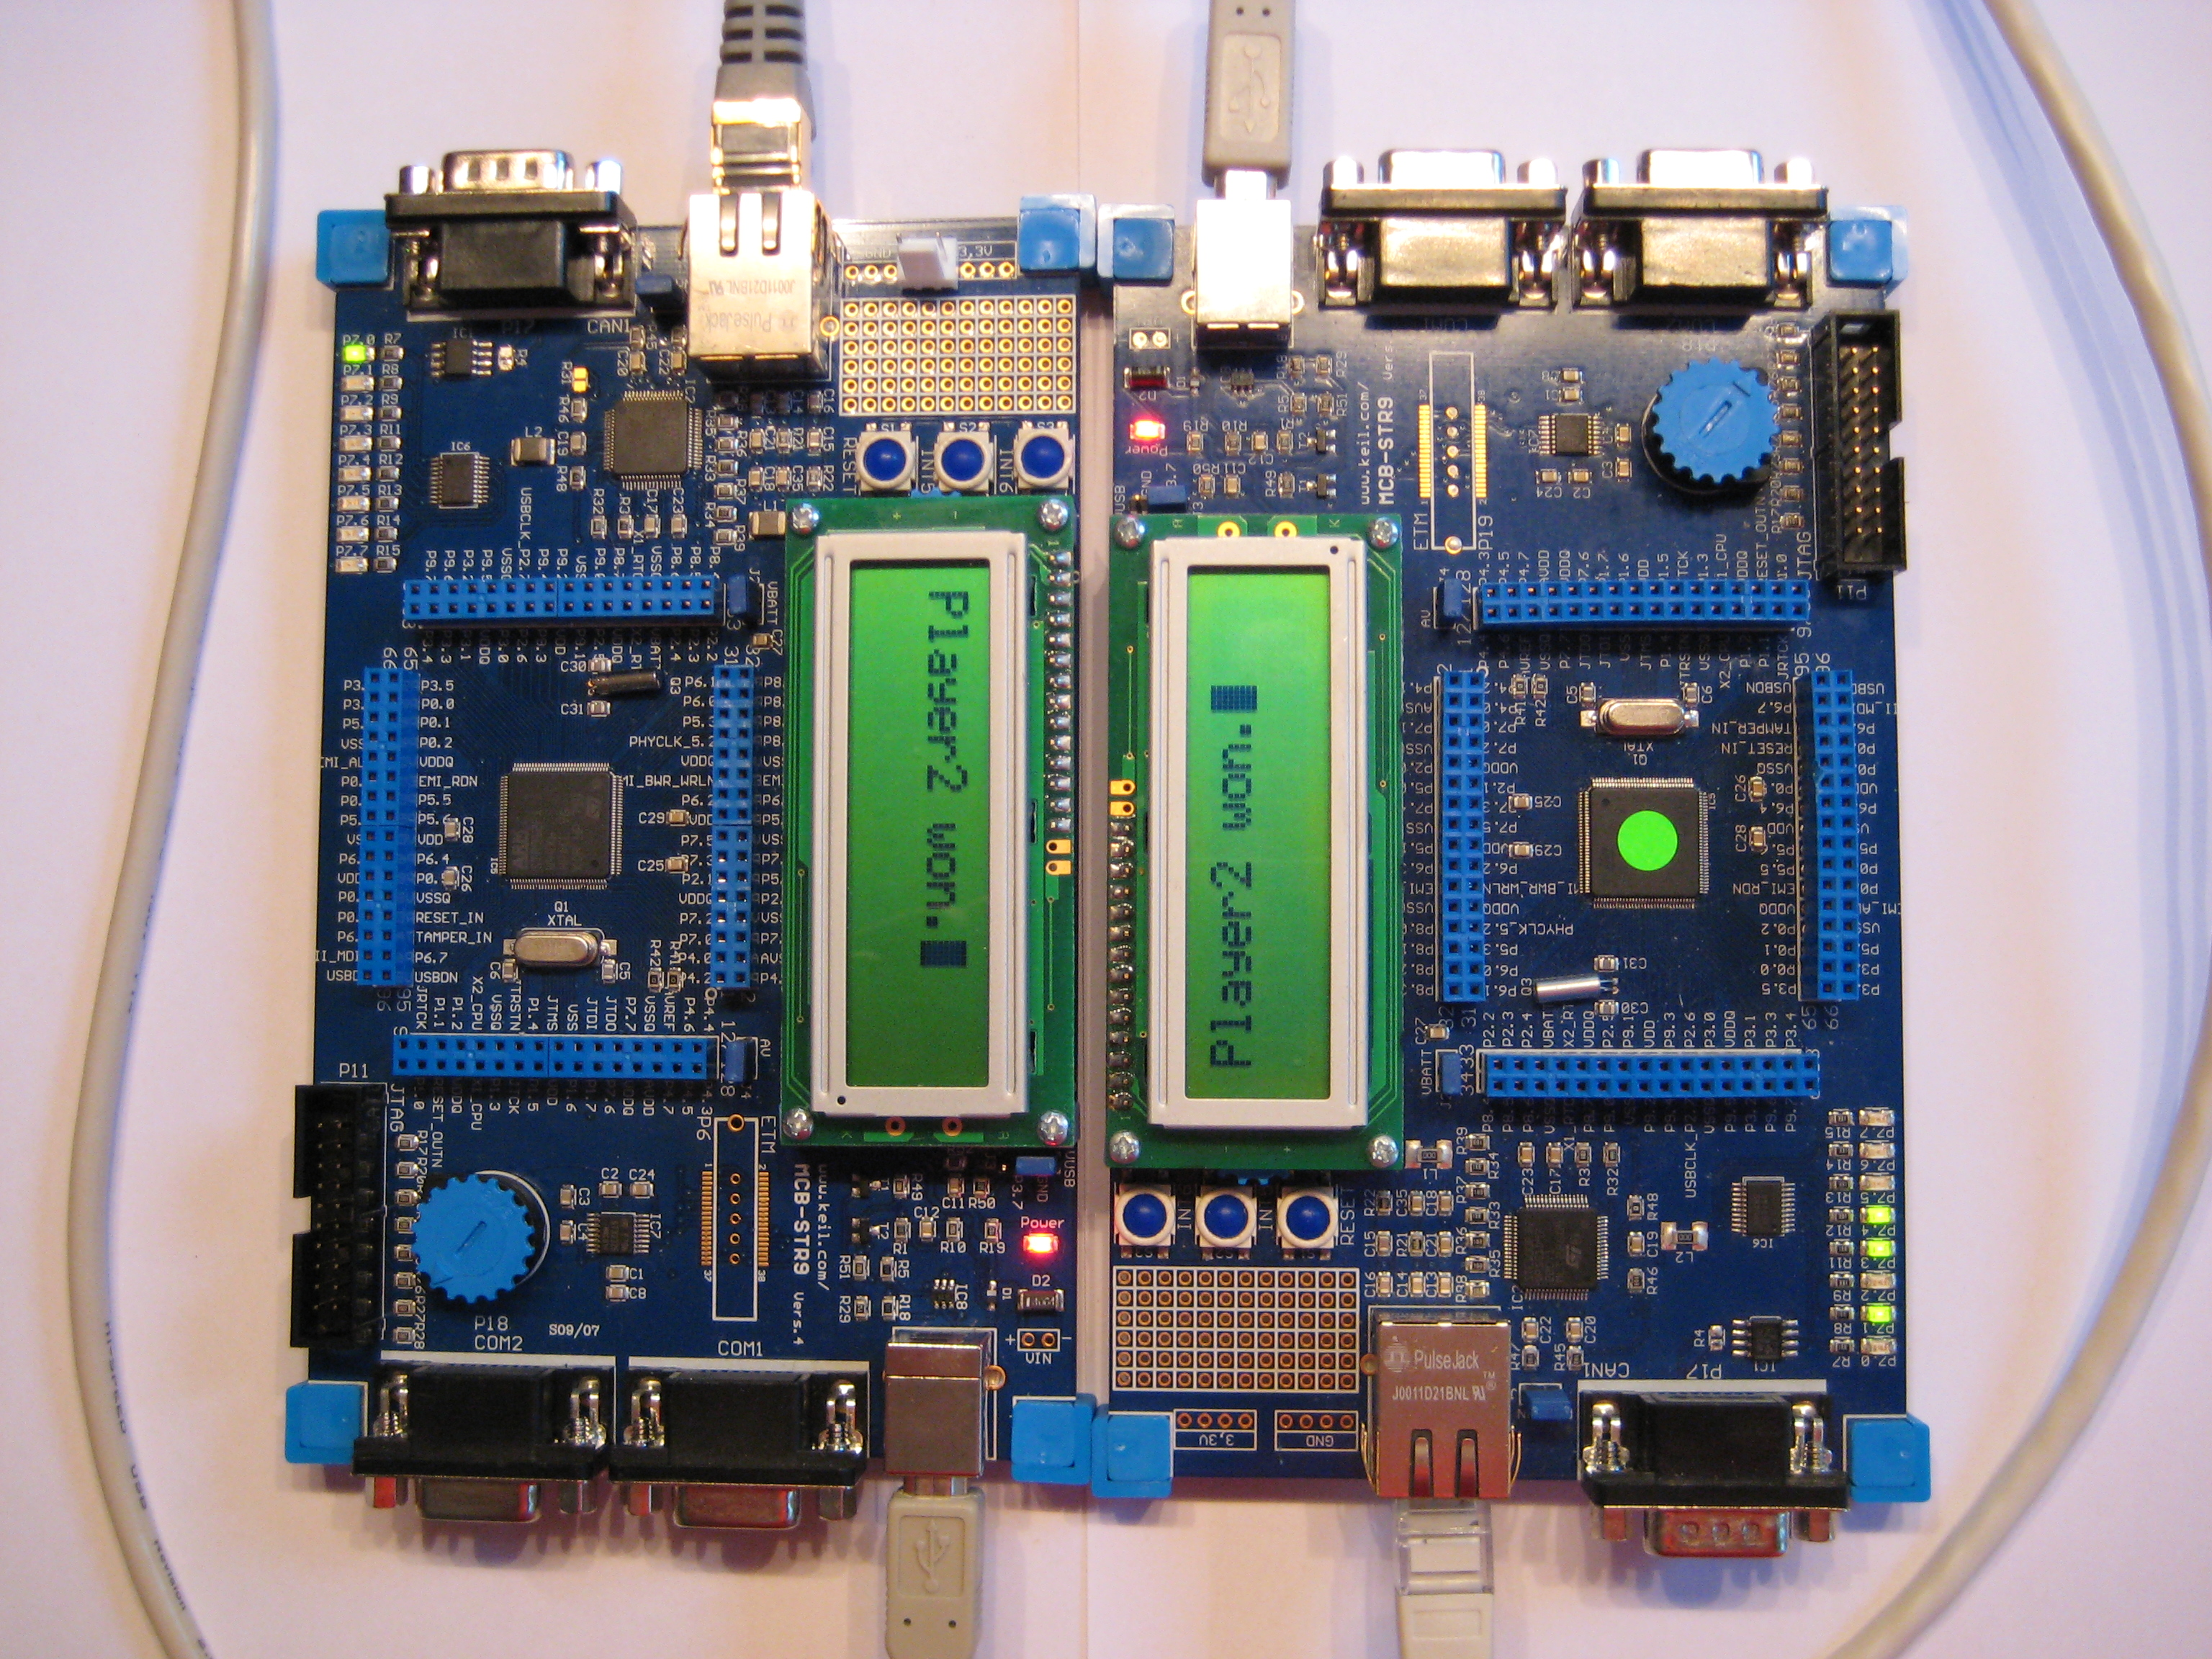
\includegraphics[width=\textwidth]{\imgPrefix/pic1.jpg}
	\caption{Hardware Setup}
	\label{fig_board_setup}
\end{figure}

\subsection{Booting}
After flashing the rom you should first start the server board. Then start the
client. As soon as booth boards are up and running the game starts. So be
ready for the challenge.

\subsection{Howto Play}
A player can interact (go left/go right with pong) with the potentiometer by
turning the wheel to the left or the right. 

\subsection{Game Rulez}
The game rulez of the pong video game are simple. The first player who let the
ball hit the wall behind the pong looses the game. 

\subsection{Status LEDs}
Keil STR9x board only. The GPIO7 leds are used to give feedback of the program
state to the user. 
\begin{itemize}
  \item GPIO0: On if Master
  \item GPIO1: On if Slave
  \item GPIO2:
  \item GPIO3: shows network action
  \item GPIO4: shows network action
  \item GPIO5:
  \item GPIO6:
  \item GPIO7: blinks if program is running
\end{itemize}

\subsection{Screenshots and Videos}
A video of the game can be found in the doc folder. 
\begin{figure}[h!]%tp]
	\centering
	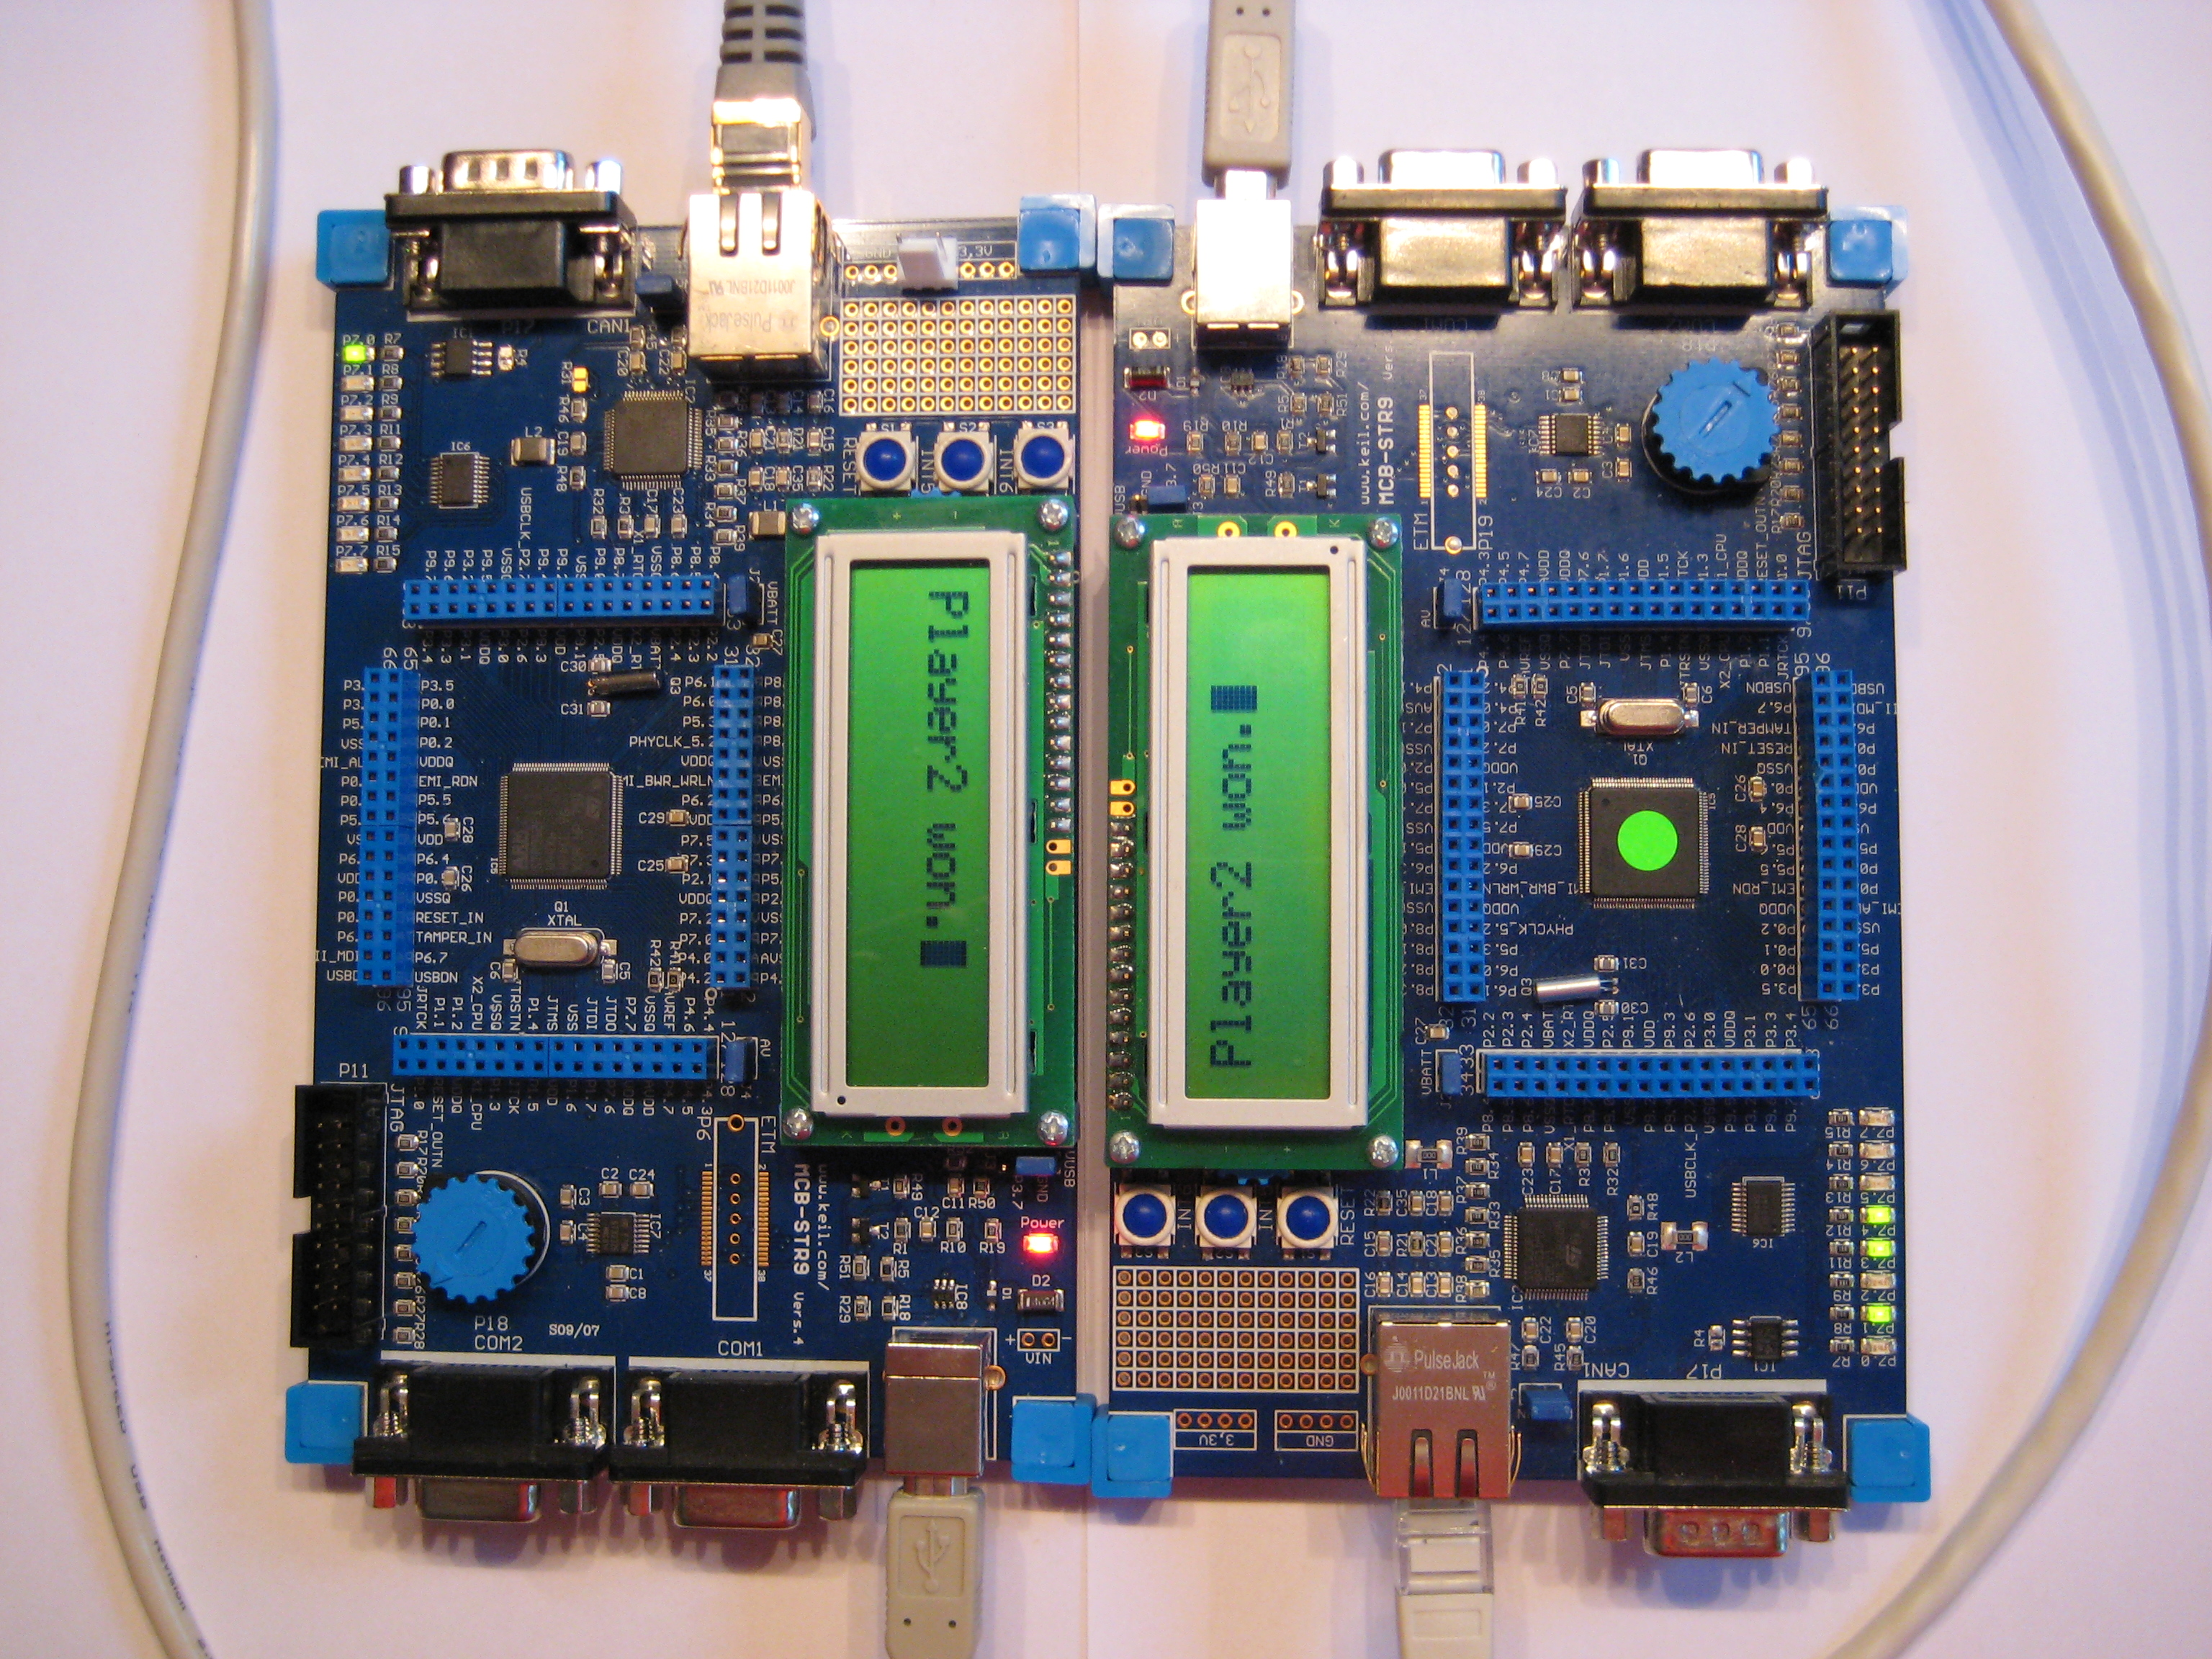
\includegraphics[width=\textwidth]{\imgPrefix/pic1.jpg}
	\caption{Demo rendering}
\end{figure}

\newpage
\section{Improvements}
The current implementation is very basic. Further simple improvements like
\begin{itemize}
  \item Alternating ball speed
  \item Improved pong steering
  \item \ldots
\end{itemize}
would make the game much more fun to play.
As always in software projects the code documentation is not perfect.
   

\newpage
\section{Conclusion}
Hardware close programming is very time consuming. It took the project team a
long time to figure out how to build the network related stuff for the game.
This was a really pain in the ass. Especially because the team used a
network stack implementation for the STR9 board that is more or less ``a
hack'' and thus is very sensible to ie. order of header file include, operation
count between network related calls and the like. 

\end{document}
